\documentclass[a4paper, 11pt]{article}

\usepackage[utf8]{inputenc}
\usepackage[slovene,english]{babel}
\usepackage[pdftex]{graphicx}
\usepackage{babelbib}
\usepackage[dvipsnames]{xcolor}
\usepackage{multirow}
\usepackage{subcaption}  % za več slik vzporedno ali vertikalno

\newcommand{\todo}{\textcolor{BrickRed}{\texttt{TODO}}} % za TODOje pisat

\makeatletter
\newcommand\tablesize{\@setfontsize\tablesize{8.5}{10.5}} % velikost med small in tiny, fajn za tabele
\makeatother

\title{Pomnenje s kvantnimi celičnimi avtomati}
\author{Jasmina Pegan, Blaž Rojc}

\begin{document}
\maketitle

\renewcommand{\figurename}{Slika} % ker Babel ne kooperira iz nekega razloga - more bit tle!

\section{Uvod}

Kvantne celice, osnovni gradniki kvantnih celičnih avtomatov, same po sebi ne omogočajo pomnenja \cite{janez_phd}.
Podobno kot pri tranzistorjih mora načrtovalec digitalnega vezja sestaviti strukturo iz kvantnih celic, ki pomnenje omogoči.
V tem delu bomo predstavili principe pomnenja v kvantnih celičnih avtomatih in nekatere strukture iz kvantnih celic, ki simulirajo delovanje tradicionalnih pomnilnih celic.



\section{Pregled področja}

\subsection{Kvantni celični avtomati}

\todo: kaka citacija? šel sem po Janežu + Mrazu

Kvantni celični avtomati predstavljajo izvedbo celičnih avtomatov, v katerih so osnovni gradniki kvantne celice.
Kvantna celica je konstrukt kvadratne oblike, ki vsebuje štiri okrogle kvantne pike in štiri tunele.
Vsak tunel povezuje dve sosednji kvantni piki.
Shema takšne celice je prikazana na sliki \ref{img-pregled-single-cell}.

\begin{figure}[h]
	\centering
	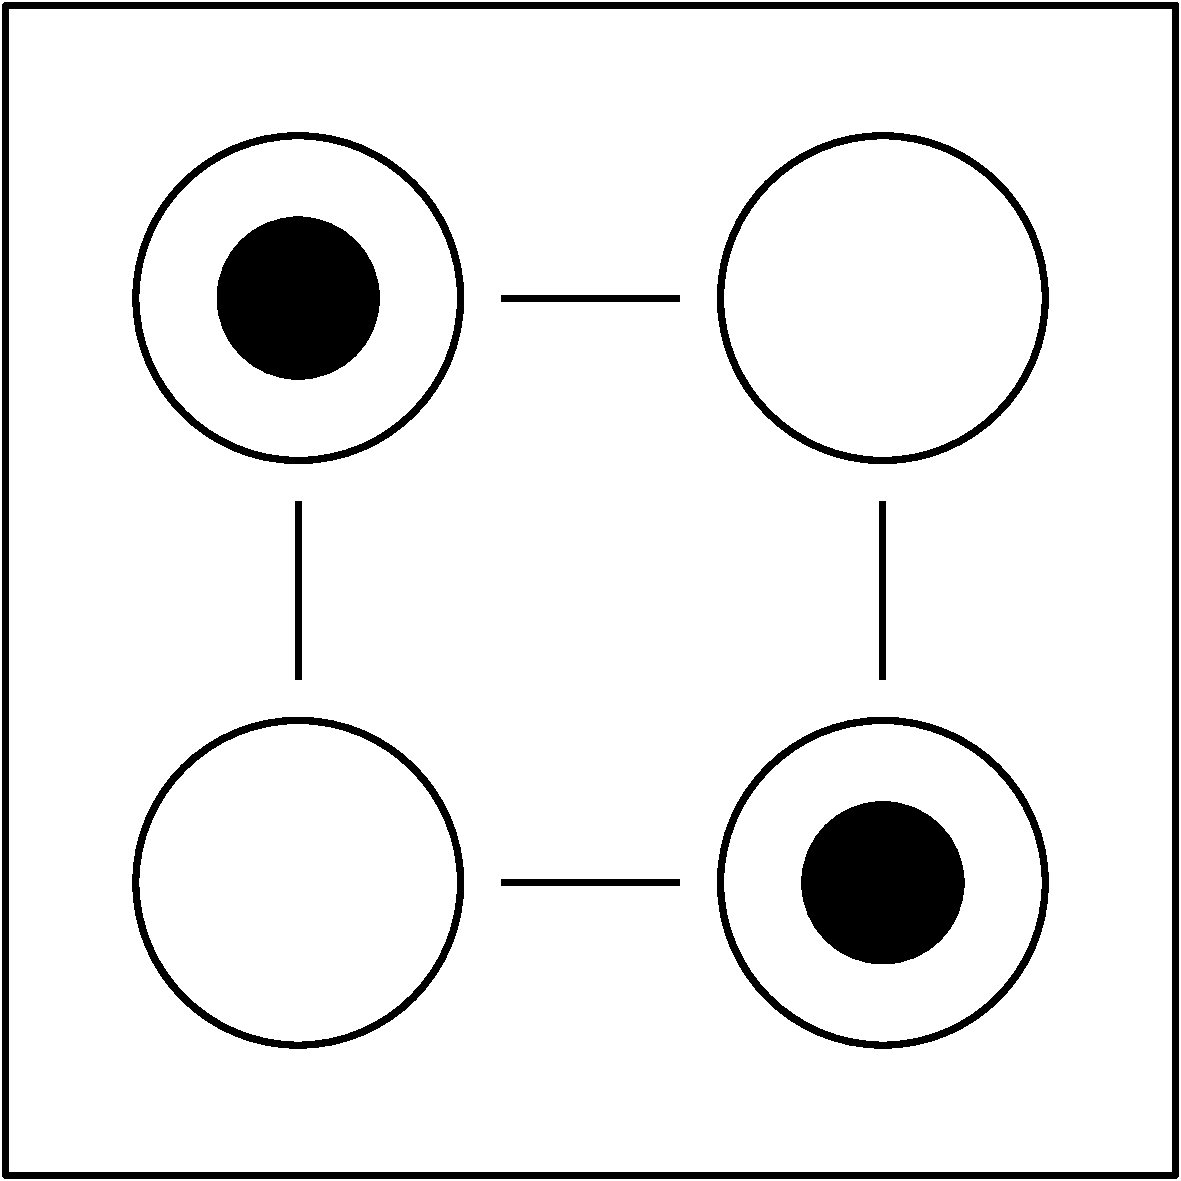
\includegraphics[width=0.35\textwidth]{../img/pregled/single_cell.pdf}
	\caption{Shema kvantne celice. Poleg štirih kvantnih pik in tunelov sta prikazana še dva elektrona, ki se nahajata v piki levo zgoraj in v piki desno spodaj.}
	\label{img-pregled-single-cell}
\end{figure}

V kvantni celici sta ujeta dva elektrona.
Vsak od njiju se lahko nahaja v eni izmed štirih kvantnih pik, med katerimi se lahko pomika prek tunelov, ki jih povezujejo.
Elektrona se zaradi odbojnih sil med njima v odsotnosti zunanjih vplivov postavita v eno izmed dveh stabilnih stanj, prikazanih na sliki \ref{img-pregled-2states}.

\begin{figure}[h]
	\centering
	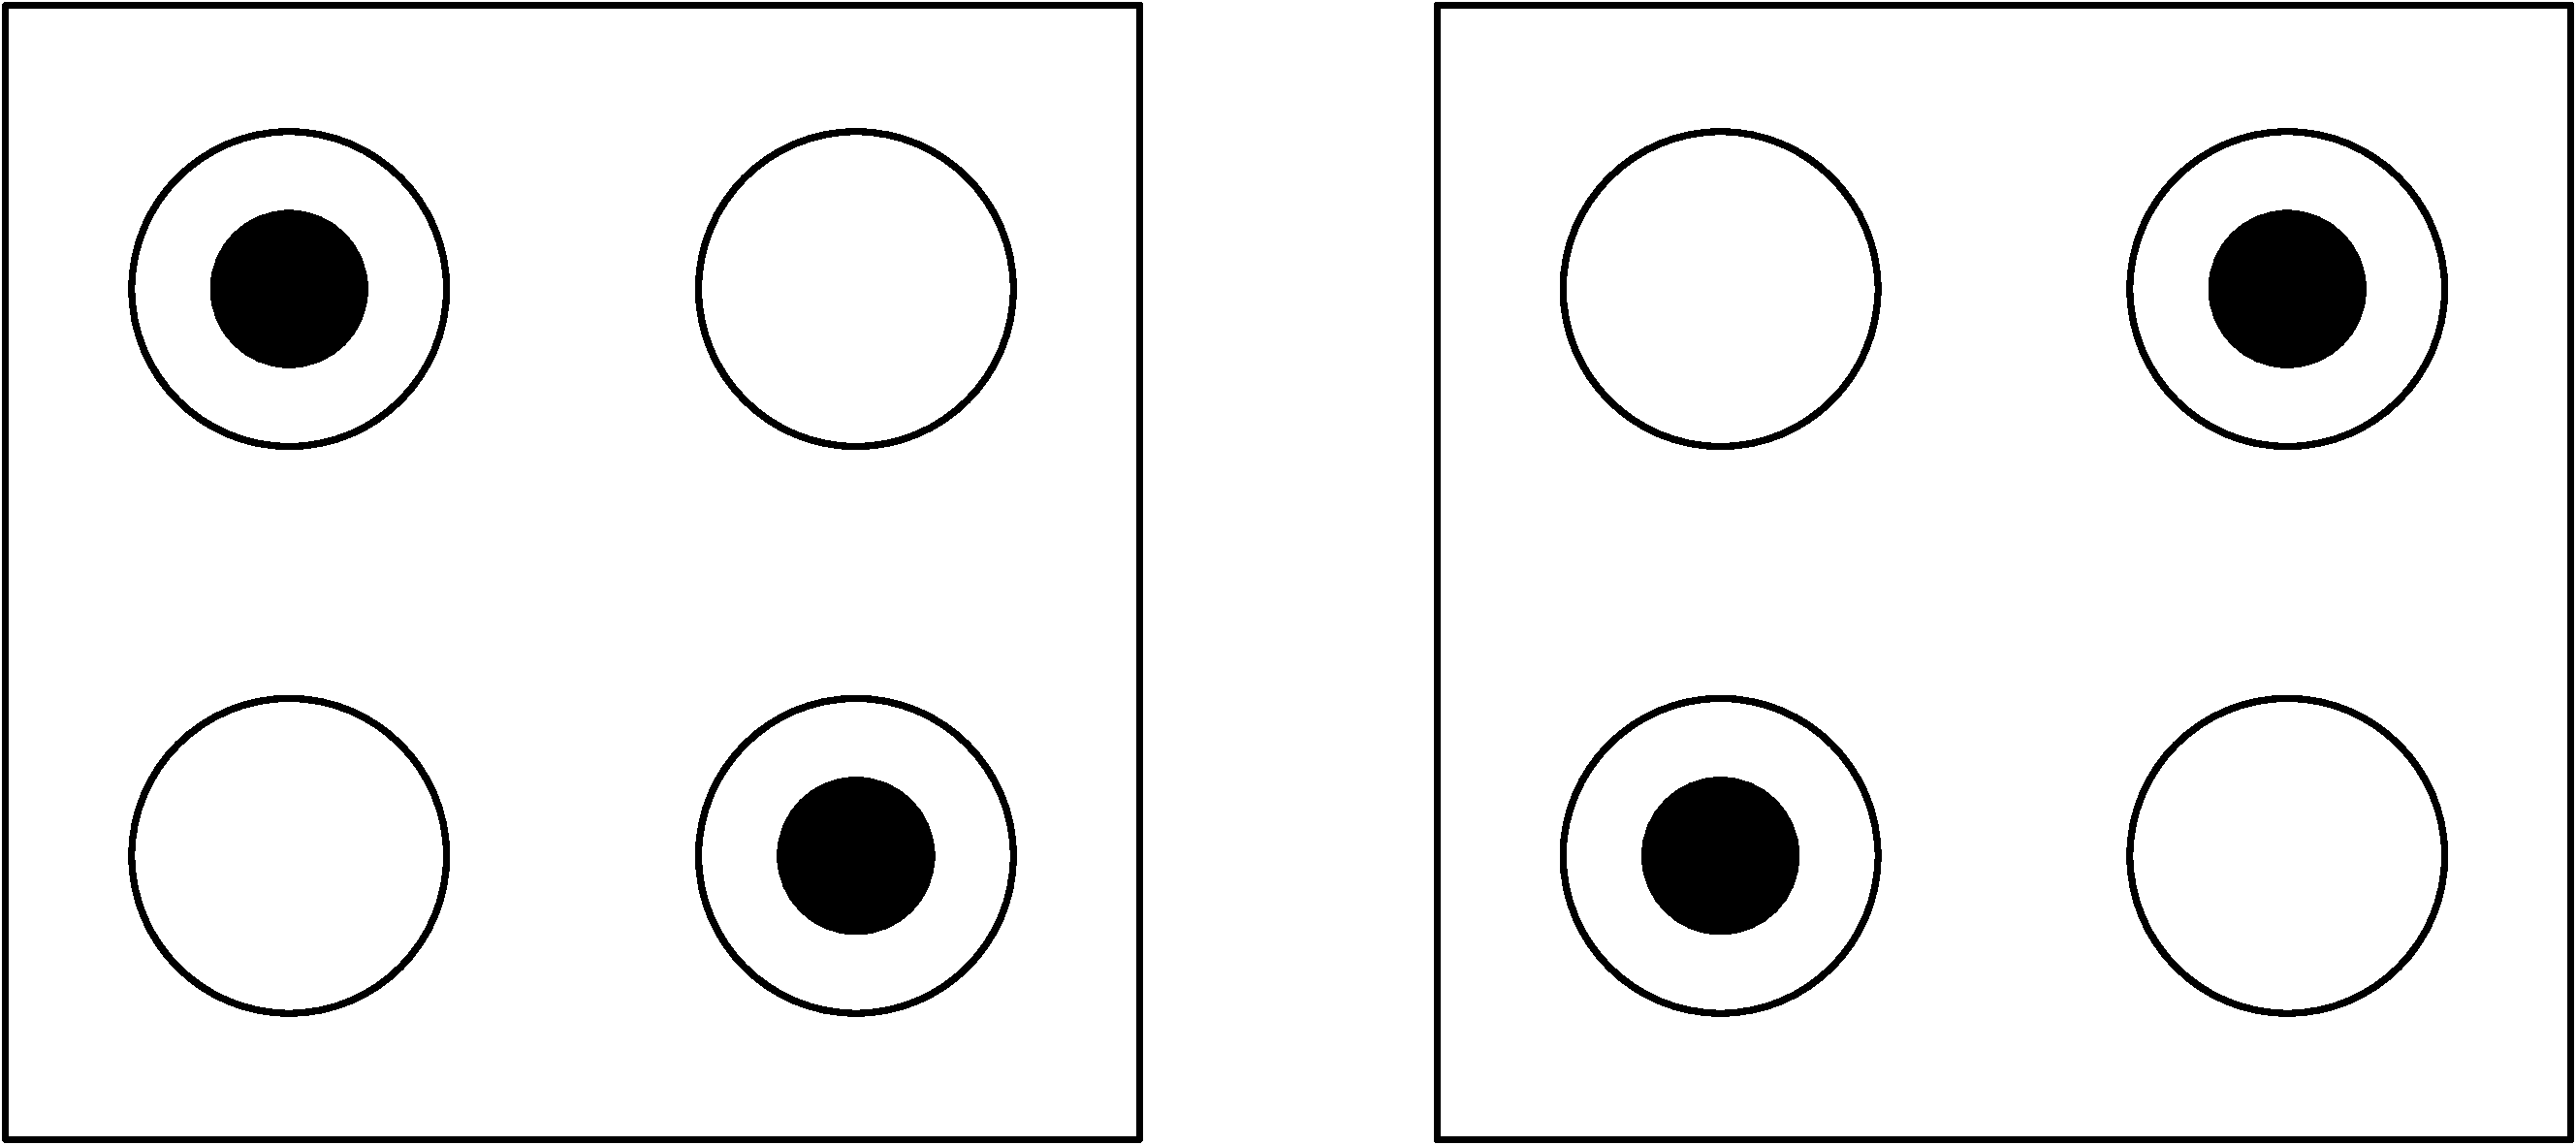
\includegraphics[width=0.65\textwidth]{../img/pregled/2states.pdf}
	\caption{Stabilni stanji kvantne celice. Na levi je prikazano stanje $P = -1$, na desni pa stanje $P = 1$.}
	\label{img-pregled-2states}
\end{figure}

Stanje $P = -1$ interpretiramo kot logično vrednost $0$, stanje $P = 1$ pa kot logično vrednost $1$ \cite{lent_1993}.
Tuneli med pikami so opremljeni s pregradami.
Elektrona lahko prosto prehajata med pikami, dokler pregrade niso vzpostavljene.
Vzpostavitev pregrad prehajanje elektronov onemogoči, kar nam omogoča, da stanje celice odčitamo.
Take celice označujemo kot izhodne.
Celico lahko tudi prisilimo, da zasede določeno stanje.
Take celice označujemo kot vhodne.

Kvantni celični avtomat je konstrukt, ki vsebuje eno ali več kvantnih celic, ki zaradi medsebojne bližine interaktirajo druga z drugo.
Sile med elektroni težijo k vzpostavitvi stanja z najmanjšo skupno energijo.
V odsotnosti zunanjih sil se kvantna celica postavi v eno izmed dveh stabilnih stanj z verjetnostjo $\frac{1}{2}$, ampak če so v njeni bližini druge kvantne celice, se ta verjetnost spremeni.
S pravilno postavitvijo celic lahko dosežemo, da se avtomat obnaša kot tradicionalna Boolova preklopna funkcija.

Gradnjo kompleksnejših struktur pričnemo z osnovnimi gradniki.
Osnovni gradniki predstavljajo poln funkcijski nabor, s katerim lahko implementiramo poljubno preklopno funkcijo.
Najenostavnejši gradnik je vodilo, prikazano na sliki \ref{img-pregled-bus}. \\*

\begin{figure}[h]
	\centering
	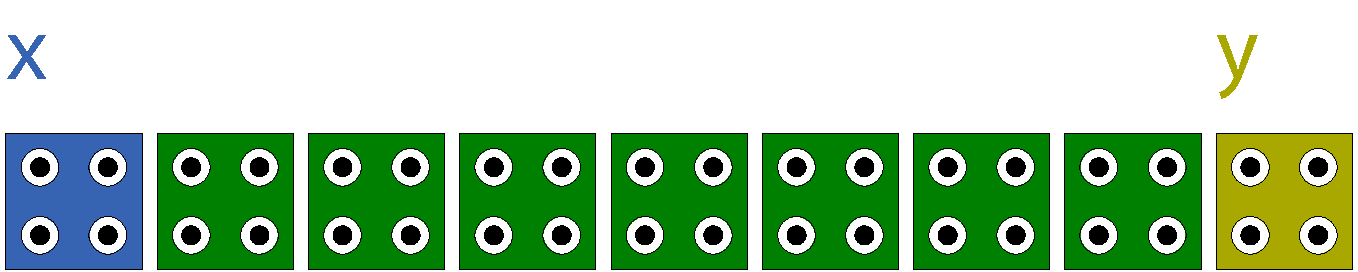
\includegraphics[width=0.75\textwidth]{../img/pregled/bus.pdf}
	\caption{Vodilo. Signal potuje od vhoda $x$ do izhoda $y$.}
	\label{img-pregled-bus}
\end{figure}

Vodila preslikajo vhodno vrednost na izhod.
Uporabljamo jih za povezovanje gradnikov v avtomatu.
Drugi gradnik je negator, prikazan na sliki \ref{img-pregled-negator}.

\begin{figure}[h]
	\centering
	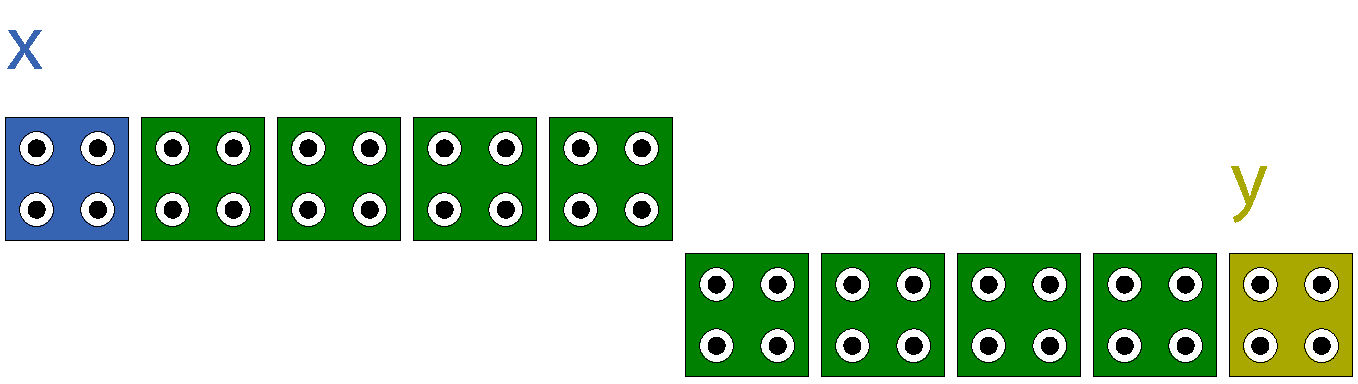
\includegraphics[width=0.75\textwidth]{../img/pregled/negator.pdf}
	\caption{Negator. Signal potuje od vhoda $x$ do izhoda $y$ in je pri tem negiran.}
	\label{img-pregled-negator}
\end{figure}

Negatorje lahko uporabimo tudi kot diagonalno vodilo, kjer je dolžina takega vodila sodo število.
Primer take uporabe je prikazan na sliki \ref{img-pregled-negbus}.

\begin{figure}[h]
	\centering
	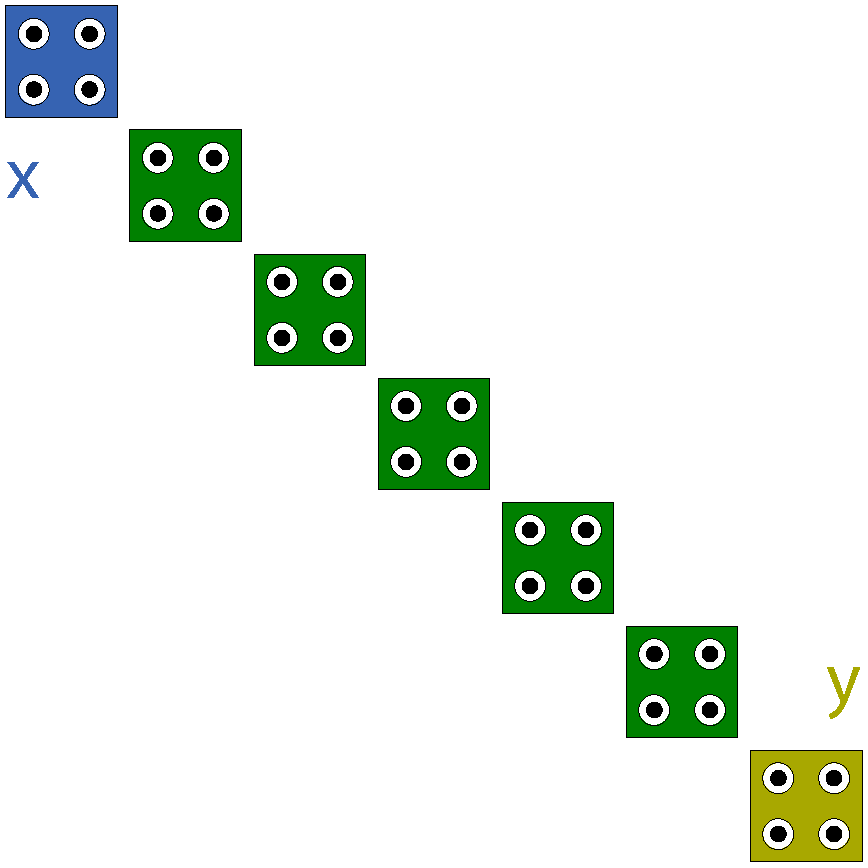
\includegraphics[width=0.45\textwidth]{../img/pregled/negbus.pdf}
	\caption{Vodilo iz negatorjev. Signal potuje od vhoda $x$ do izhoda $y$. Pri tem je negiran $2k$-krat, zato se logična vrednost ne spremeni.}
	\label{img-pregled-negbus}
\end{figure}

Zadnji osnovni gradnik so večinska oz.~majoritetna vrata, prikazana na sliki \ref{img-pregled-major}.

\begin{figure}[h]
	\centering
	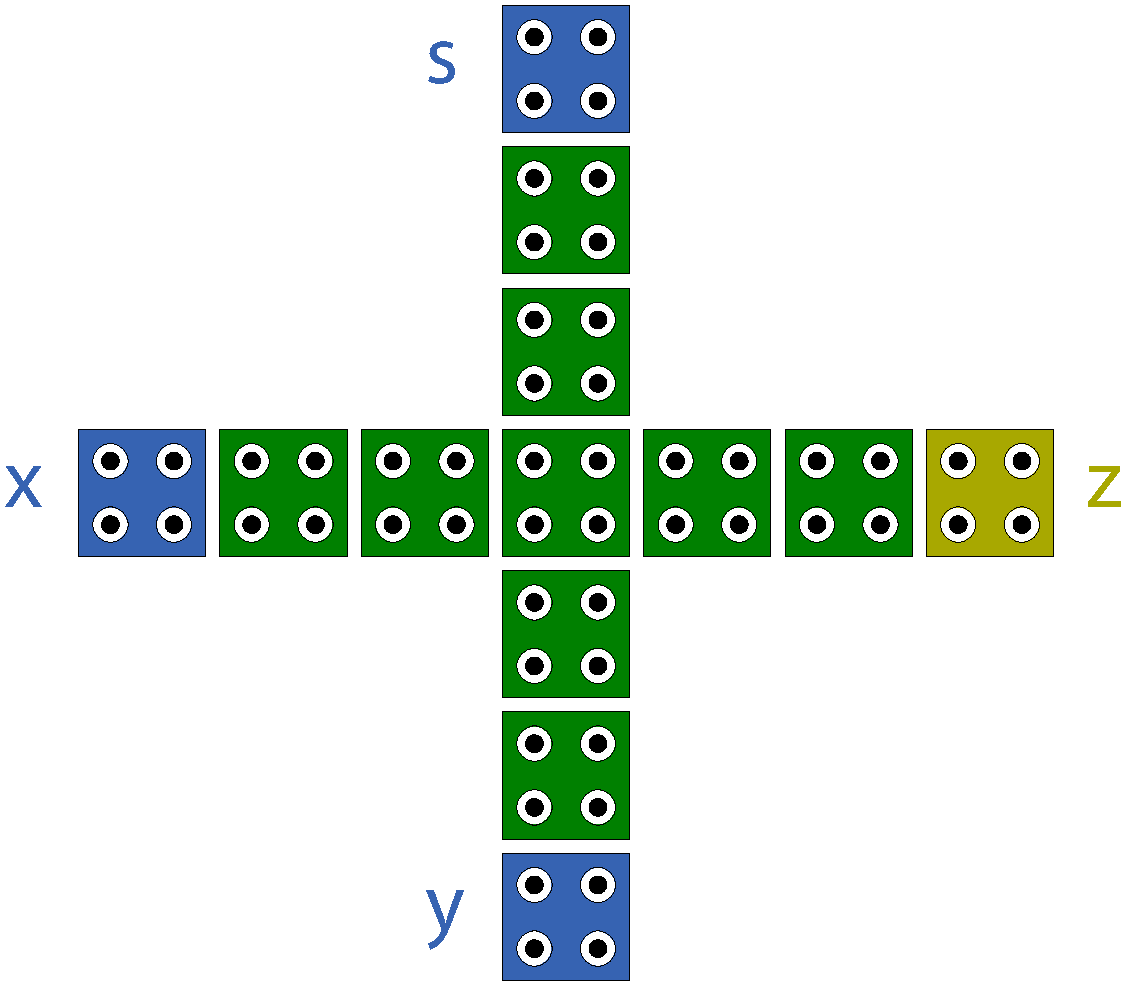
\includegraphics[width=0.55\textwidth]{../img/pregled/major.pdf}
	\caption{Majoritetna vrata. Izhod $z$ zavzame večinsko vrednost na vhodih $s$, $x$ in $y$.}
	\label{img-pregled-major}
\end{figure}

Izhod majoritetnih vrat zavzame večinsko vrednost na treh vhodih.
Z vezavo konstante na enega izmed vhodov majoritetnih vrat dobimo gradnik, ki predstavlja konjunkcijo ali disjunkcijo, kot je prikazano na sliki \ref{tab-pregled-major}.

\begin{figure}
	\centering
	\small
	\begin{tabular}{c|c|c||c c}
	$s$ & $x$ & $y$ & $z$ \\
	\hline
	$0$ & $0$ & $0$ & $0$ & \multirow{4}{*}{$AND(x, y)$} \\
	$0$ & $0$ & $1$ & $0$ \\
	$0$ & $1$ & $0$ & $0$ \\
	$0$ & $1$ & $1$ & $1$ \\
	\hline
	$1$ & $0$ & $0$ & $0$ & \multirow{4}{*}{$OR(x, y)$} \\
	$1$ & $0$ & $1$ & $1$ \\
	$1$ & $1$ & $0$ & $1$ \\
	$1$ & $1$ & $1$ & $1$ \\
	\end{tabular}
	\caption{Tabela vrednosti izhoda majoritetnih vrat pri različnih vhodnih vrednostih. Majoritetna vrata se glede na $x$ in $y$ pri $s = 0$ obnašajo kot konjunkcija, pri $s = 1$ pa kot disjunkcija.}
	\label{tab-pregled-major}
\end{figure}

Tok podatkov v avtomatu usmerjamo s pomočjo urinih con.
Vsaki celici dodelimo eno izmed štirih urinih con, ki se ciklično izmenjujejo.
Tako omogočimo logično separacijo delov avtomata in način interakcije med njimi.

\subsection{Problematika pomnenja}

Ko je ura odsotna, je stanje kvantne celice v odsotnosti zunanjih sil nedeterministično.
Tako kvantnih celic samih ne moremo uporabiti za hrambo podatkov.
Uvedba ure omogoča, da kvantne celice spravimo v zaklenjeno stanje, v katerem prehajanje elektronov med pikami ni mogoče, kar pomeni, da je stanje zaklenjene kvantne celice deterministično.
Za pomnenje potrebujemo še način za nadzor stanja, ki naj ga zaklenjena celica zavzame.
To lahko dosežemo z veriženjem celic, ki ne pripadajo isti urini coni.
Takšna veriga je prikazana na sliki \ref{img-pregled-seq-linear}.

\begin{figure}[h]
	\centering
	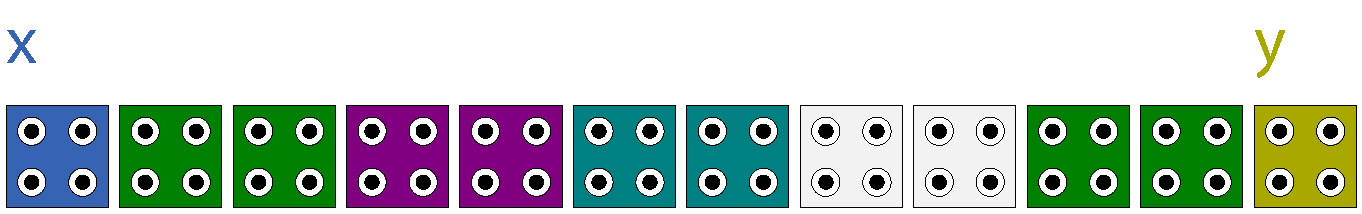
\includegraphics[width=0.75\textwidth]{../img/pregled/seq_linear.pdf}
	\caption{Veriga kvantnih celic s sekvenčnimi urinimi conami. Različne barve celic, ki niso vhodne ali izhodne, označujejo različne urine cone.}
	\label{img-pregled-seq-linear}
\end{figure}

Za samostojno pomnenje to verigo sklenemo v obroč, prikazan na sliki \ref{img-pregled-seq-circ}.
V obroču se stanje med potekom urinega cikla ohranja.
Za smiselno uporabo želimo to strukturo prirediti tako, da lahko hranjeno stanje poljubno nastavljamo.
Kako to storimo, je stvar implementacije.
V nadaljevanju bomo predstavili nekaj obstoječih implementacij pomnilnih struktur.

\begin{figure}[h]
	\centering
	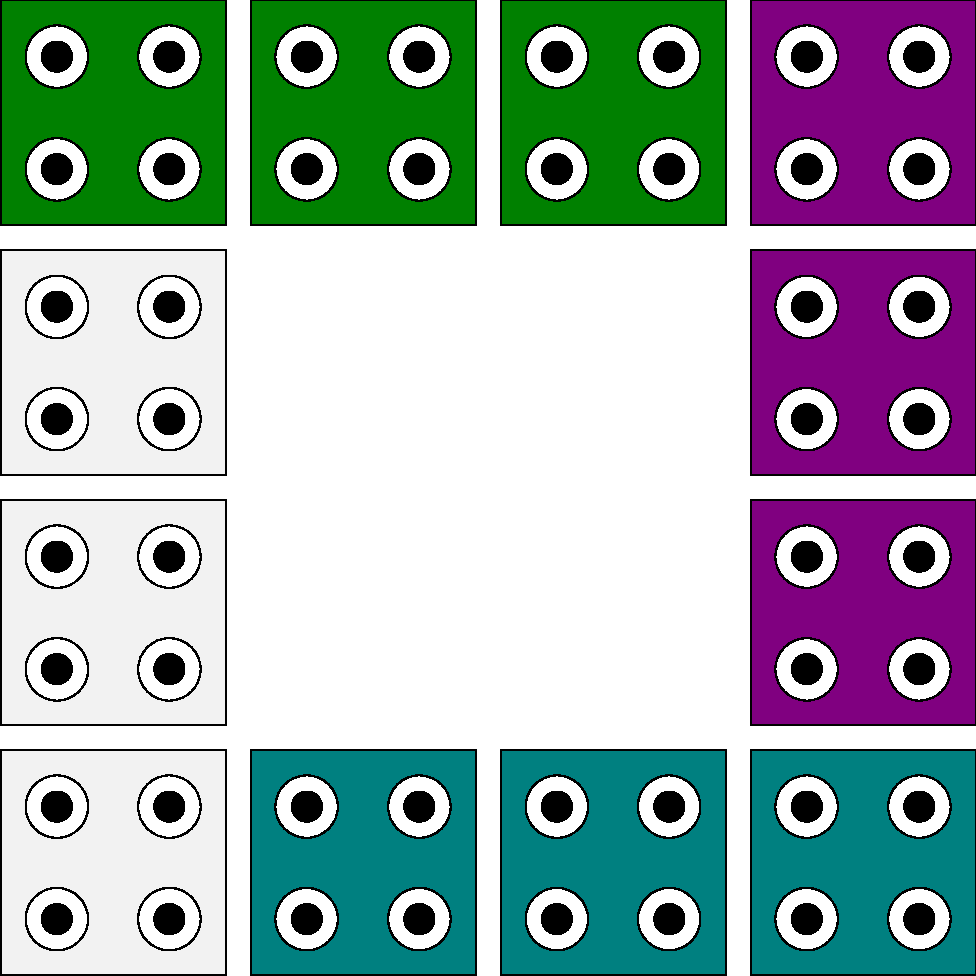
\includegraphics[width=0.40\textwidth]{../img/pregled/seq_circ.pdf}
	\caption{Obroč kvantnih celic s sekvenčnimi urinimi conami. Tak obroč sam po sebi ni uporaben, saj ne vsebuje vhodnih in izhodnih celic.}
	\label{img-pregled-seq-circ}
\end{figure}



\section{Pomnilne celice}
Za gradnjo sekvenčnih vezij poleg logičnih vrat potrebujemo tudi pomnilne celice.
Osnovne pomnilne celice, ki omogočajo hranjenje enega bita informacije, so RS (Reset Set), JK (Jump Kill), T (Trigger) in D (Delay) pomnilna celica.
Delovanje pomnilnih celic je podano v tabelah na sliki \ref{tab-cells-table}.

\begin{figure}[h]
	\centering
	\tablesize
	\begin{tabular}{cccc}
		
		\begin{tabular}{c|c|c||c}
		$r$ & $s$ & $q$ & $D^1q$ \\
		\hline
		\hline
		$0$ & $0$ & $0$ & $0$ \\
		$0$ & $0$ & $1$ & $1$ \\
		\hline
		$0$ & $1$ & $0$ & $1$ \\
		$0$ & $1$ & $1$ & $1$ \\
		\hline
		$1$ & $0$ & $0$ & $0$ \\
		$1$ & $0$ & $1$ & $0$ \\
		\hline
		$1$ & $1$ & $0$ & \textcolor{Red}{$\times$} \\
		$1$ & $1$ & $1$ & \textcolor{Red}{$\times$} \\
		\end{tabular}
		
		&
		
		\begin{tabular}{c|c|c||c}
		$j$ & $k$ & $q$ & $D^1q$ \\
		\hline
		\hline
		$0$ & $0$ & $0$ & $0$ \\
		$0$ & $0$ & $1$ & $1$ \\
		\hline
		$0$ & $1$ & $0$ & $1$ \\
		$0$ & $1$ & $1$ & $1$ \\
		\hline
		$1$ & $0$ & $0$ & $0$ \\
		$1$ & $0$ & $1$ & $0$ \\
		\hline
		$1$ & $1$ & $0$ & $1$ \\
		$1$ & $1$ & $1$ & $0$ \\
		\end{tabular}
		
		&
		
		\begin{tabular}{c|c||c}
		$t$ & $q$ & $D^1q$ \\
		\hline
		\hline
		$0$ & $0$ & $0$ \\
		$0$ & $1$ & $1$ \\
		\hline
		$1$ & $0$ & $1$ \\
		$1$ & $1$ & $0$ \\
		\end{tabular}
		
		&
		
		\begin{tabular}{c|c||c}
		$d$ & $q$ & $D^1q$ \\
		\hline
		\hline
		$0$ & $0$ & $0$ \\
		$0$ & $1$ & $0$ \\
		\hline
		$1$ & $0$ & $1$ \\
		$1$ & $1$ & $1$ \\
		\end{tabular}
		
		\\ \\
		RS celica & JK celica & T celica & D celica \\
	\end{tabular}
	\caption{Pravilnostne tabele pomnilniških celic. \textcolor{Red}{$\times$} predstavlja nedovoljeno stanje.}
	\label{tab-cells-table}
\end{figure}


\subsection{Obstoječe implementacije}
V članku \cite{quantum_dot} iz leta 2003 so predstavljene implementacije štirih osnovnih pomnilnih celic. Vse celice porabijo en urin cikel za procesiranje vhodov. Pri postavitvi celic vir uporablja pravilo čimbolj preprostih oblik urinih con in čimmanj le-teh. Po drugi strani pa so nekatere celice zasukane za kot $ 45^{\circ} $ ali zamaknjene za polovico svoje velikosti, kar lahko negativno vpliva na izvedljivost implementacije. Vir uporablja križanje linij, kar je možno doseči z uporabo alternirajočega vodila (rotiranih celic). \\

Vse implementacije pomnilnih celic v viru \cite{a_novel_approach} iz leta 2018 temeljijo na izpeljavah izraza, ki opisuje RS celico. Te implementacije porabijo manj celic ter ponudijo tako izhodno stanje $Q$ kot njegovo negacijo $\bar{Q}$, so pa zato urine cone bolj kompleksne in uporabljeni so manj stabilni negatorji kot v prvem viru. Vse celice se izvedejo v $1.5$ urinega cikla, le D pomnilna celica ima latenco $1.25$ urinega cikla.

%\subsection{Reverzibilne implementacije (?)}

\subsection{Ideje in popravki (?)}
\todo: sploh damo to?
\begin{itemize}
\item Uporaba večjih razdalj med gradniki
\item Konsistentna uporaba bolj stabilne negacije
\end{itemize}

\section{Implementacija}
\todo: primerjaj implementacije: potratnost, izvedljivost, konsistentnost\\
V tem poglavju bomo primerjali predlagane implementacije pomnilnih celic.\\

V viru \cite{a_novel_approach} so enačbe posameznih pomnilnih celic izpeljane iz enačb RS celice:
\begin{equation}
Qb = \overline{\overline{B \cdot CLK} \cdot Q} = B \cdot CLK + \overline{Q},
\label{eq-rs-qb}
\end{equation}
\begin{equation}
Q = \overline{\overline{A \cdot CLK} \cdot Qb} = A \cdot CLK + \overline{Qb} = A \cdot CLK + \overline{B \cdot CLK} \cdot Q,
\label{eq-rs-q}
\end{equation}
pri čemer je $Q$ izhod celice, $Qb$ njegova negacija, $A$ in $B$ sta vhoda ter $CLK$ je vhodni urin signal.

\begin{table}[h!]
\tablesize
\begin{tabular}{|c|c|c|c|c|}
\hline 
Pomnilna celica & Vir & Število majoritetnih vrat & Število negatorjev & Število celic \\ 
\hline 
\multirow{2}{*}{D} & \cite{quantum_dot} & 3 & 2 & 68 \\ 
& \cite{a_novel_approach} & 4 & 2 & 43 \\ 
\hline 
\multirow{2}{*}{JK} & \cite{quantum_dot} & 5 & 2 & 90 \\ 
& \cite{a_novel_approach} & 6 & 2 & 78 \\ 
\hline 
\multirow{2}{*}{RS} & \cite{quantum_dot} & 4 & 1 & 76 \\ 
& \cite{a_novel_approach} & 4 & 2 & 38 \\ 
\hline 
\multirow{2}{*}{T} & \cite{quantum_dot} & 5 & 4 & 92 \\  
& \cite{a_novel_approach} & 6 & 2 & 81 \\ 
\hline 
\end{tabular}
\caption{Primerjava števila gradnikov za sestavo pomnilnih celic.} 
\label{st-gradnikov}
\end{table}

\subsection{D pomnilna celica}
Na sliki \ref{fig-d} vidimo implementaciji D pomnilne celice po obeh virih. Vir \cite{quantum_dot} uporabi križanje linij urinega signala in vhoda $D$ z uporabo alternirajočega vodila zasukanih celic. Vir \cite{a_novel_approach} v enačbah \ref{eq-rs-qb} in \ref{eq-rs-q} zamenja vhoda $A$ in $B$ z $D$ in $\overline{D}$ ter tako dobi enačbo D pomnilne celice.

\begin{figure}[h!]
	\begin{subfigure}[b]{0.5\textwidth}
	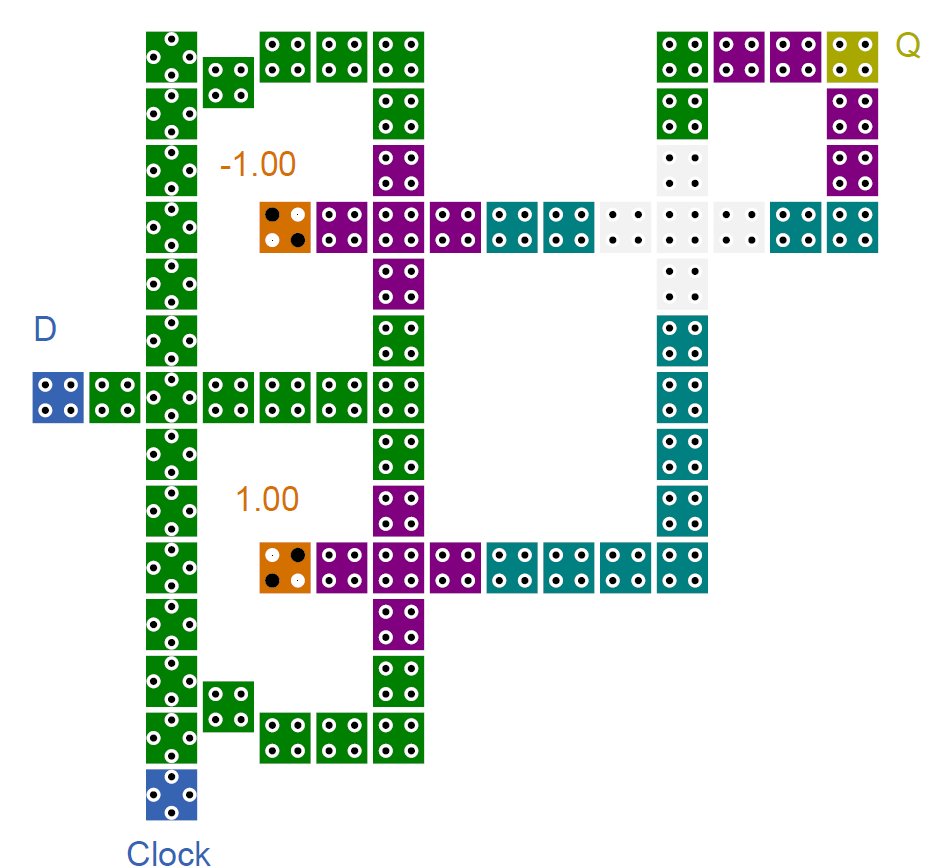
\includegraphics[width=\textwidth]{../img/vir_4/d.png}
	\caption{D pomnilna celica po viru \cite{quantum_dot}}
	\label{fig-d-1}
	\end{subfigure}
	\begin{subfigure}[b]{0.5\textwidth}
	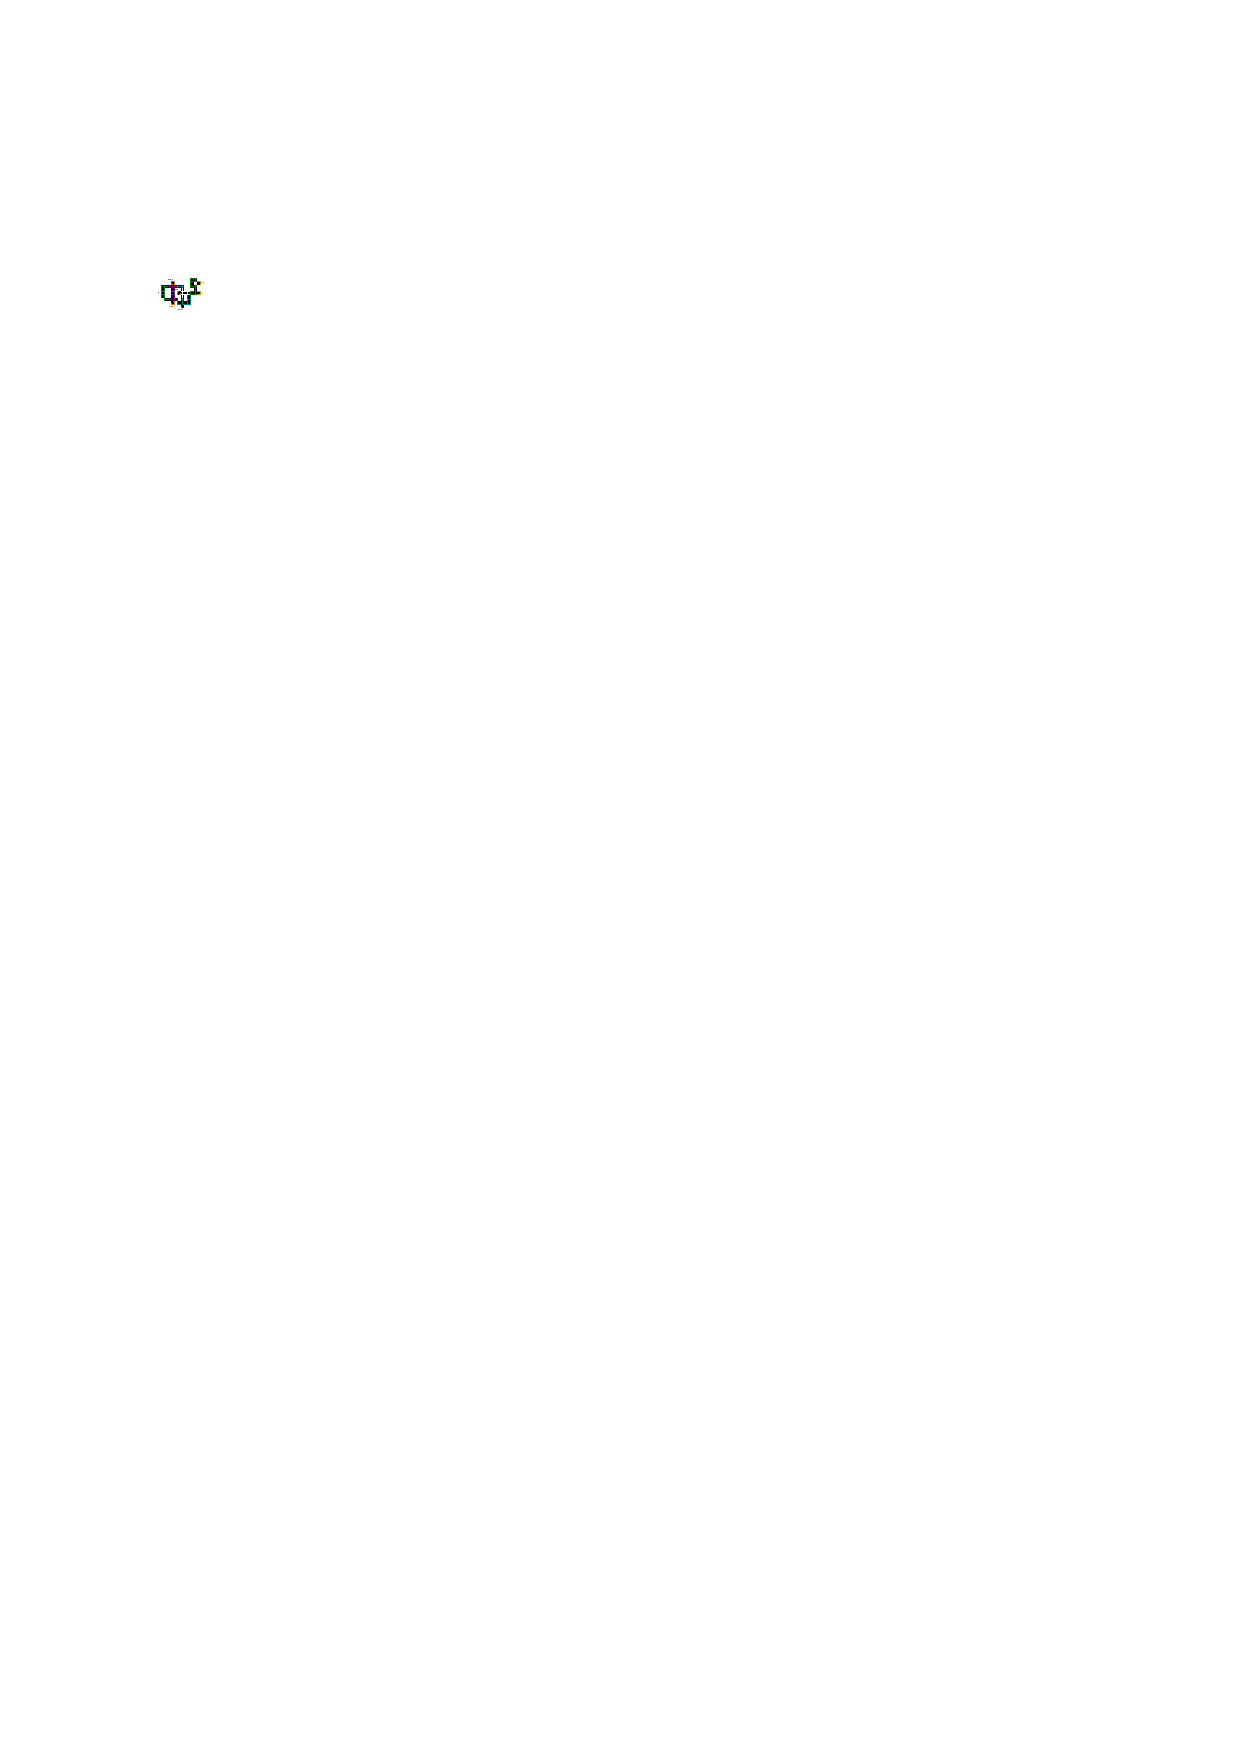
\includegraphics[width=\textwidth]{../img/vir_5/d.png} 
	\caption{D pomnilna celica po viru \cite{a_novel_approach}}
	\label{fig-d-2}
	\end{subfigure}
	\caption{Implementaciji D pomnilne celice}
	\label{fig-d}
\end{figure}

\subsection{JK pomnilna celica}
Na sliki \ref{fig-jk} vidimo implementaciji JK celice po obeh virih. Vir \cite{quantum_dot} uporabi alternirajoče vodilo za širjenje urinega signala za bolj stabilen prenos signala naprej, vidimo tudi dva okrepljena negatorja. Da izpelje enačbo JK pomnilne celice, vir \cite{a_novel_approach} strukturi za RS celico doda dve majoritetni vrati.
\begin{figure}[h!]
	\begin{subfigure}[b]{0.5\textwidth}
	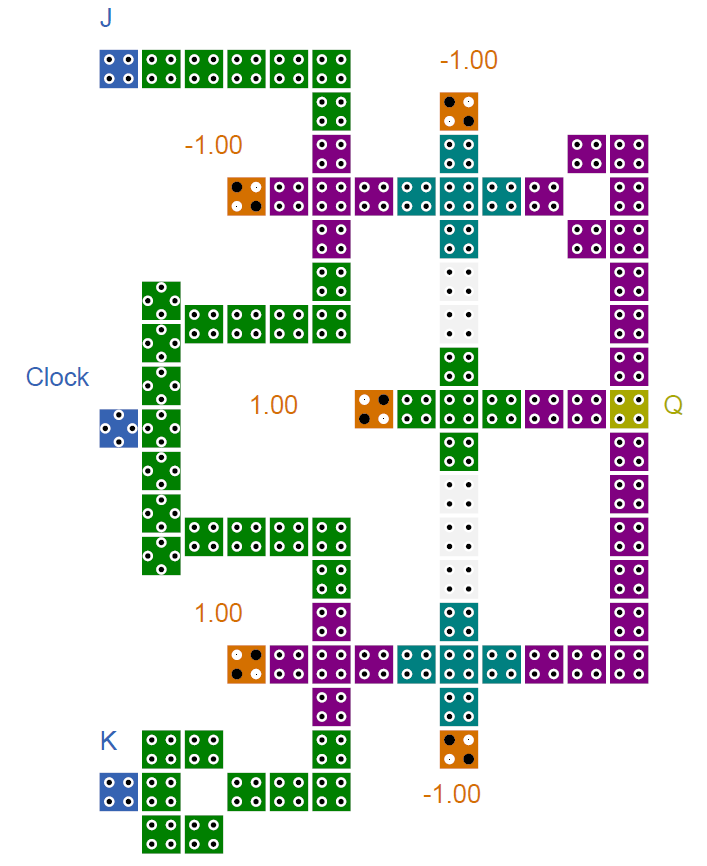
\includegraphics[width=\textwidth]{../img/vir_4/jk.png}
	\caption{JK pomnilna celica po viru \cite{quantum_dot}}
	\label{fig-jk-1}
	\end{subfigure}
	\begin{subfigure}[b]{0.5\textwidth}
	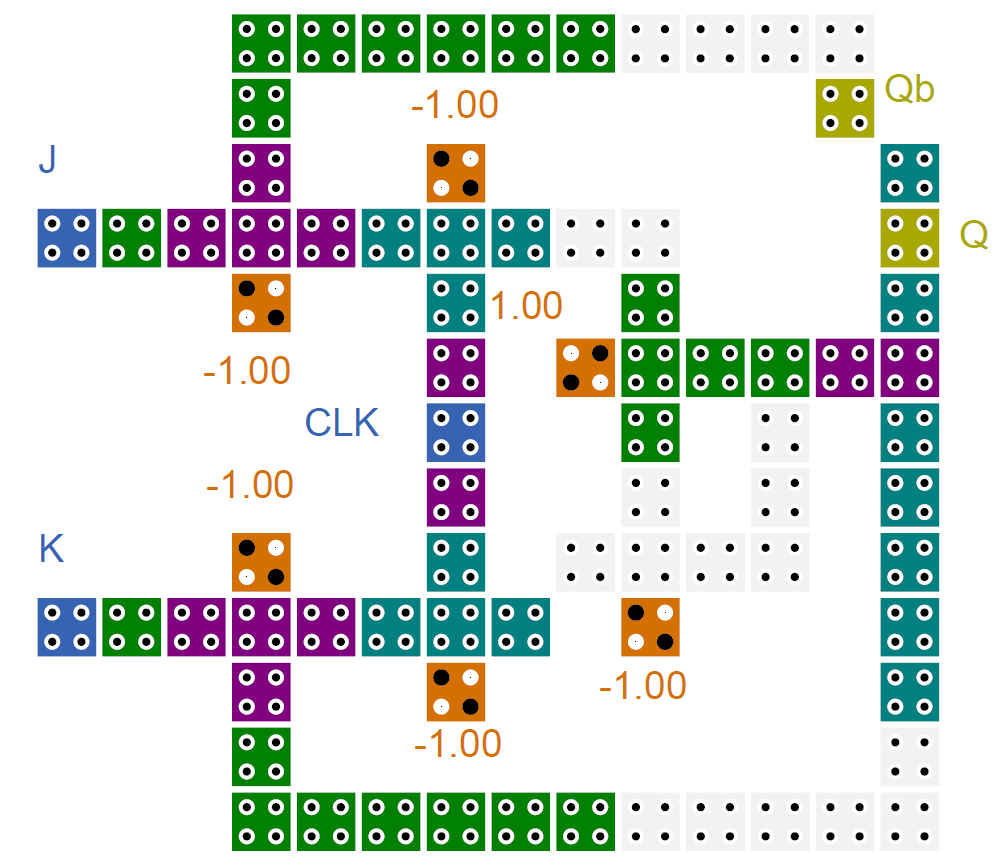
\includegraphics[width=\textwidth]{../img/vir_5/jk.png} 
	\caption{JK pomnilna celica po viru \cite{a_novel_approach}}
	\label{fig-jk-2}
	\end{subfigure}
	\caption{Implementaciji JK pomnilne celice}
	\label{fig-jk}
\end{figure}

\subsection{RS pomnilna celica}
Na sliki \ref{fig-rs} vidimo implementaciji RS celice po obeh virih. Vir \cite{quantum_dot} kot pri JK celici uporabi alternirajoče vodilo za širjenje urinega signala in en okrepljen negator. Vir \cite{a_novel_approach} v enačbah \ref{eq-rs-qb} in \ref{eq-rs-q} zamenja vhoda $A$ in $B$ s $S$ in $R$ ter tako dobi enačbo RS pomnilne celice.
\begin{figure}[h!]
	\begin{subfigure}[b]{0.5\textwidth}
	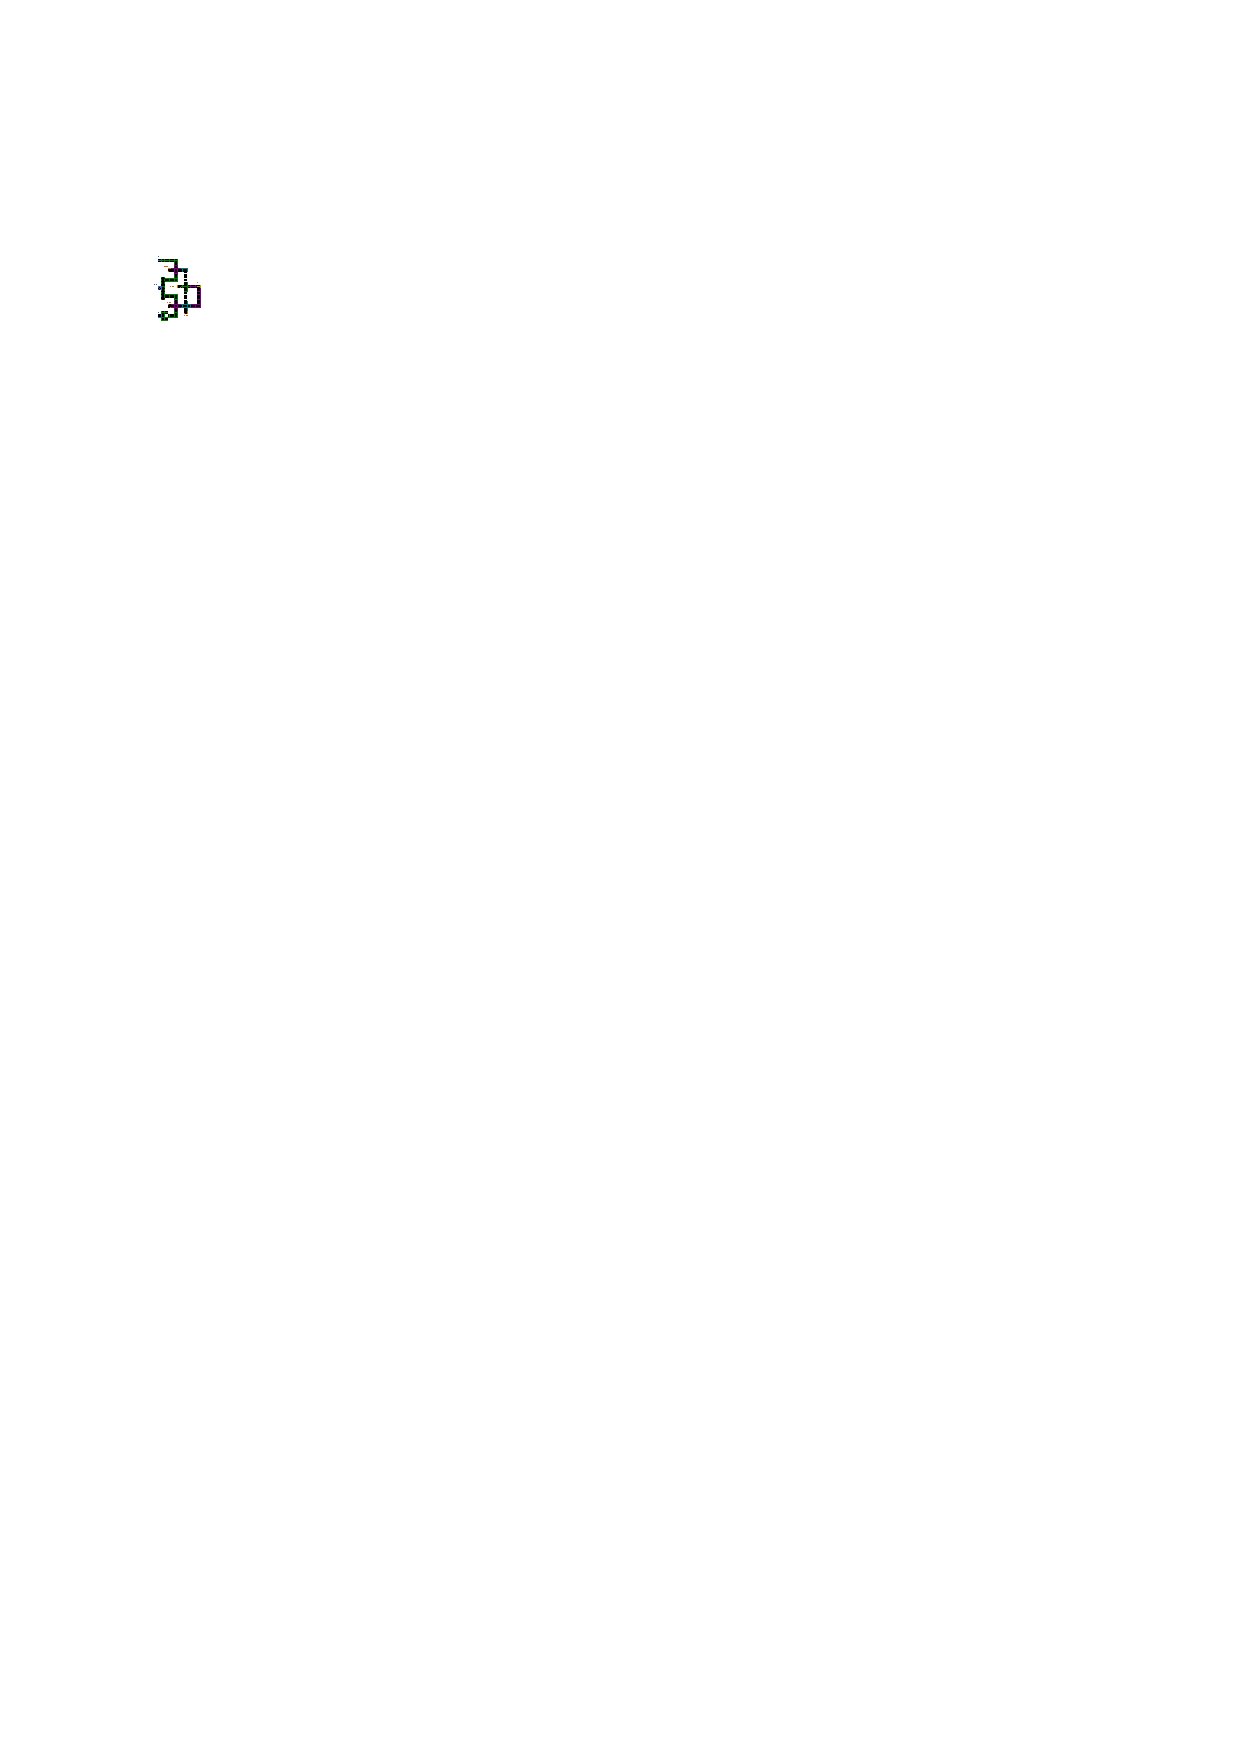
\includegraphics[width=\textwidth]{../img/vir_4/sr.png}
	\caption{RS pomnilna celica po viru \cite{quantum_dot}}
	\label{fig-rs-1}
	\end{subfigure}
	\begin{subfigure}[b]{0.5\textwidth}
	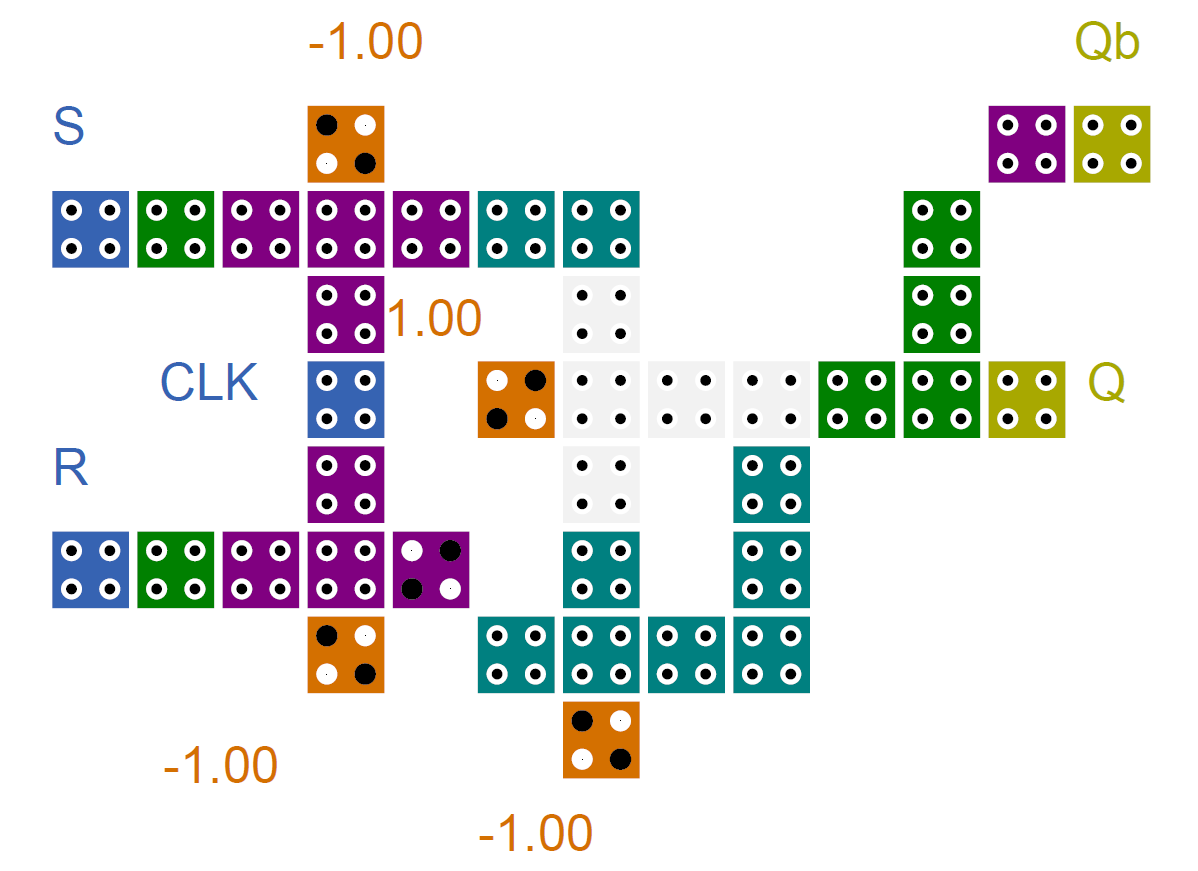
\includegraphics[width=\textwidth]{../img/vir_5/rs.png} 
	\caption{RS pomnilna celica po viru \cite{a_novel_approach}}
	\label{fig-rs-2}
	\end{subfigure}
	\caption{Implementaciji RS pomnilne celice}
	\label{fig-rs}
\end{figure}

\subsection{T pomnilna celica}
Na sliki \ref{fig-t} vidimo implementaciji T celice po obeh virih. Vir \cite{quantum_dot} spet uporabi alternirajoče vodilo za širjenje urinega signala in dva okrepljena negatorja. Tudi prenosa z alternirajočega vodila prek polovično zamaknjenih celic učinkujeta kot negatorja. Vir \cite{a_novel_approach} pridobi enačbo za T pomnilno celico iz JK pomnilne celice s povezavo vhodov $J$ in $K$.
\begin{figure}[h!]
	\begin{subfigure}[b]{0.5\textwidth}
	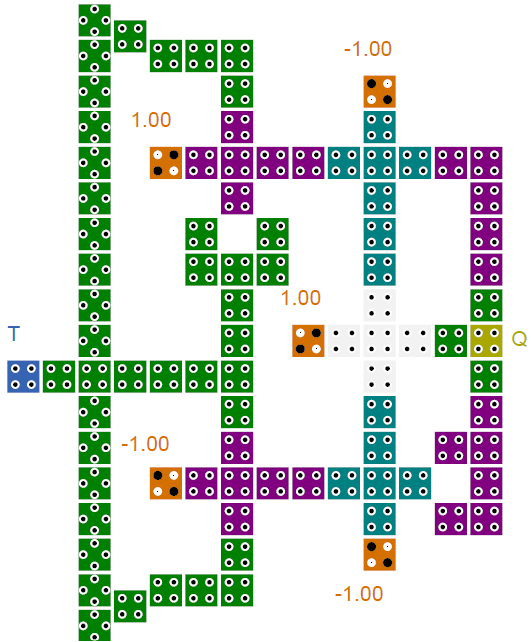
\includegraphics[width=\textwidth]{../img/vir_4/t.png}
	\caption{T pomnilna celica po viru \cite{quantum_dot}}
	\label{fig-t-1}
	\end{subfigure}
	\begin{subfigure}[b]{0.5\textwidth}
	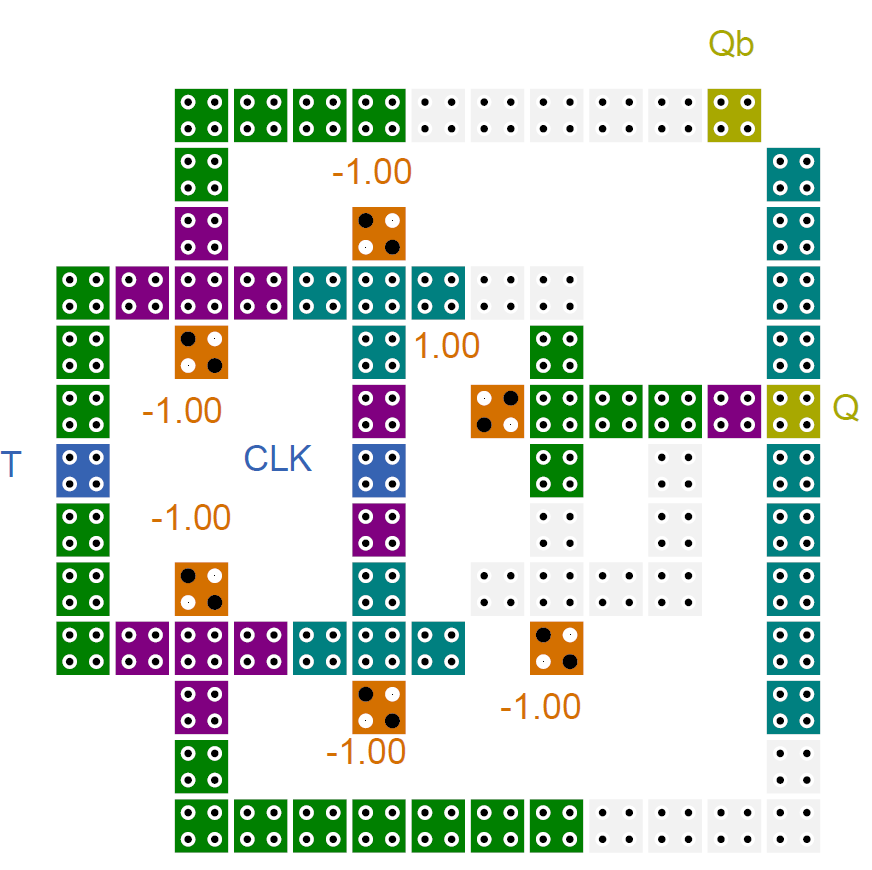
\includegraphics[width=\textwidth]{../img/vir_5/t.png} 
	\caption{T pomnilna celica po viru \cite{a_novel_approach}}
	\label{fig-t-2}
	\end{subfigure}
	\caption{Implementaciji T pomnilne celice}
	\label{fig-t}
\end{figure}


\subsection{Analiza delovanja}
V sledečem poglavju bomo analizirali rezultate simulacij pomnilnih celic in jih primerjali s pričakovanimi pravilnostnimi tabelami.

\subsubsection{D pomnilna celica}
Pravilnostna tabela D pomnilne celice je predstavljena v tabeli \ref{tab-d}.
\begin{table}[h!]
	\centering
	\small
	\begin{tabular}{c|c}
	$d$ & $D^1q$ \\
	\hline
	$0$ & $0$ \\
	$1$ & $1$ \\
	\end{tabular}
	\caption{Pravilnostna tabela D pomnilne celice.}
	\label{tab-d}
\end{table}

Na sliki \ref{fig-d-sim} vidimo obnašanje $Q$ celice v odvisnosti od vhoda $D$ in urinega signala $Clock$. Že takoj lahko vidimo, da se rezultata simulacij razlikujeta. Iz razbranega lahko sestavimo pravilnostni tabeli \ref{tab-d-sim}.
\begin{table}[h!]
	\centering
	\small
	\begin{tabular}{cc|cccc|c}
	\multicolumn{3}{c}{vir \cite{quantum_dot}} & $\quad$ & \multicolumn{3}{c}{vir \cite{a_novel_approach}}\\
	$D$ & $Clock$ & $Q$ && $D$ & $Clock$ & $Q$ \\
	\cline{1-3} \cline{5-7}
	$0$ & $0$ & $0$ && $0$ & $0$ & $1$\\
	$0$ & $1$ & $0$ && $0$ & $1$ & $0$\\
	$1$ & $0$ & $0$ && $1$ & $0$ & $0$\\
	$1$ & $1$ & $1$ && $1$ & $1$ & $0$\\
	\cline{1-3} \cline{5-7}
	$0$ & $0$ & $1$ && $0$ & $0$ & $1$\\
	$0$ & $1$ & $0$ && $0$ & $1$ & $0$\\
	$1$ & $0$ & $0$ && $1$ & $0$ & $0$\\
	$1$ & $1$ & $1$ && $1$ & $1$ & $0$\\
	\end{tabular}
	\caption{Rezultat simulacije D pomnilne celice.}
	\label{tab-d-sim}
\end{table}


\begin{figure}[h!]
	\begin{subfigure}[b]{\textwidth}
	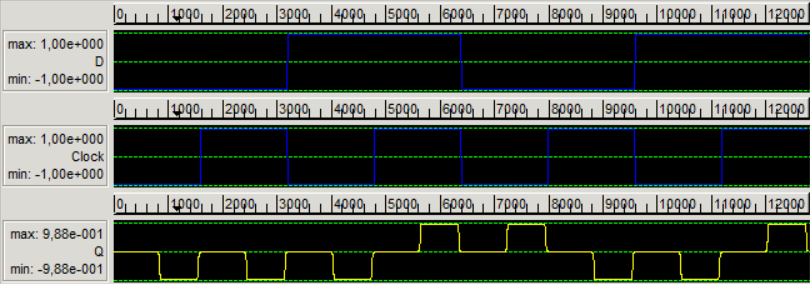
\includegraphics[width=\textwidth]{../img/vir_4/sim_d.png}
	\caption{Simulacija delovanja D pomnilne celice po viru \cite{quantum_dot}}
	\label{fig-d-1-sim}
	\end{subfigure}
	\begin{subfigure}[b]{\textwidth}
	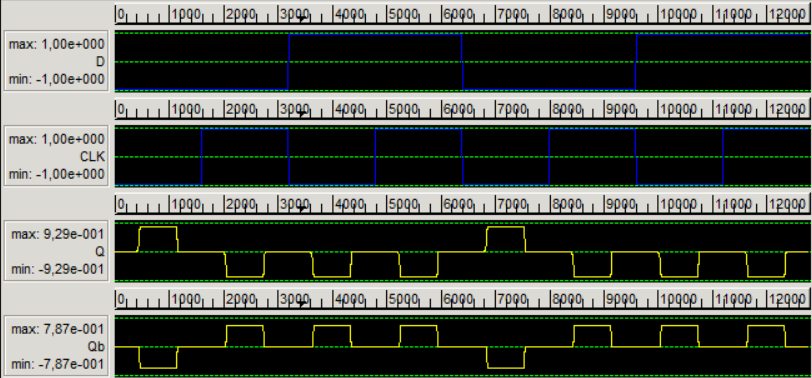
\includegraphics[width=\textwidth]{../img/vir_5/sim_d.png}
	\caption{Simulacija delovanja D pomnilne celice po viru \cite{a_novel_approach}}
	\label{fig-d-2-sim}
	\end{subfigure}
	\caption{Simulaciji D pomnilne celice}
	\label{fig-d-sim}
\end{figure}

\subsubsection{JK pomnilna celica}
Pravilnostna tabela JK pomnilne celice je predstavljena v tabeli \ref{tab-jk}.
\begin{table}[h!]
	\centering
	\small
	\begin{tabular}{cc|c}
	$k$ & $j$ & $D^1q$ \\
	\hline
	$0$ & $0$ & $q$ \\
	$0$ & $1$ & $1$ \\
	$1$ & $0$ & $0$ \\
	$1$ & $1$ & $\overline{q}$ \\
	\end{tabular}
	\caption{Pravilnostna tabela JK pomnilne celice.}
	\label{tab-jk}
\end{table}

Na sliki \ref{fig-jk-sim} vidimo obnašanje $Q$ celice v odvisnosti od vhodov $J$ in $K$ ter urinega signala $Clock$. Iz razbranega lahko sestavimo pravilnostni tabeli \ref{tab-jk-sim}.
\begin{table}[h!]
	\centering
	\small
	\begin{tabular}{ccc|ccccc|c}
	\multicolumn{4}{c}{vir \cite{quantum_dot}} & $\quad$ & \multicolumn{4}{c}{vir \cite{a_novel_approach}}\\
	$J$ & $Clock$ & $K$ & $Q$ && $J$ & $Clock$ & $K$ & $Q$ \\
	\cline{1-4} \cline{6-9}
	$0$ & $0$ & $0$ & $1$ && $0$ & $0$ & $0$ & $0$\\
	$0$ & $0$ & $1$ & $1$ && $0$ & $0$ & $1$ & $0$\\
	$0$ & $1$ & $0$ & $1$ && $0$ & $1$ & $0$ & $0$\\
	$0$ & $1$ & $1$ & $1$ && $0$ & $1$ & $1$ & $0$\\
	$1$ & $0$ & $0$ & $1$ && $1$ & $0$ & $0$ & $0$\\
	$1$ & $0$ & $1$ & $1$ && $1$ & $0$ & $1$ & $0$\\
	$1$ & $1$ & $0$ & $1$ && $1$ & $1$ & $0$ & $0$\\
	$1$ & $1$ & $1$ & $0$ && $1$ & $1$ & $1$ & $1$\\
	\cline{1-4} \cline{6-9}
	$0$ & $0$ & $0$ & $1$ && $0$ & $0$ & $0$ & $1$\\
	$0$ & $0$ & $1$ & $1$ && $0$ & $0$ & $1$ & $0$\\
	$0$ & $1$ & $0$ & $1$ && $0$ & $1$ & $0$ & $0$\\
	$0$ & $1$ & $1$ & $1$ && $0$ & $1$ & $1$ & $0$\\
	$1$ & $0$ & $0$ & $1$ && $1$ & $0$ & $0$ & $0$\\
	$1$ & $0$ & $1$ & $1$ && $1$ & $0$ & $1$ & $0$\\
	$1$ & $1$ & $0$ & $1$ && $1$ & $1$ & $0$ & $0$\\
	$1$ & $1$ & $1$ & $0$ && $1$ & $1$ & $1$ & $1$\\
	\end{tabular}
	\caption{Rezultat simulacije JK pomnilne celice.}
	\label{tab-jk-sim}
\end{table}

\begin{figure}[h!]
	\begin{subfigure}[b]{\textwidth}
	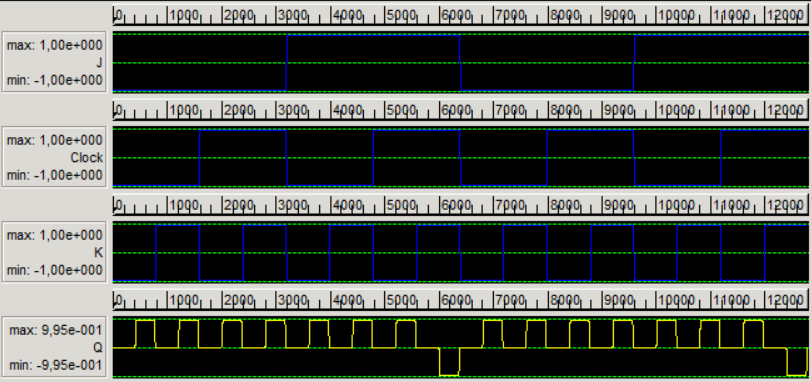
\includegraphics[width=\textwidth]{../img/vir_4/sim_jk.png}
	\caption{Simulacija delovanja JK pomnilne celice po viru \cite{quantum_dot}}
	\label{fig-jk-1-sim}
	\end{subfigure}
	\begin{subfigure}[b]{\textwidth}
	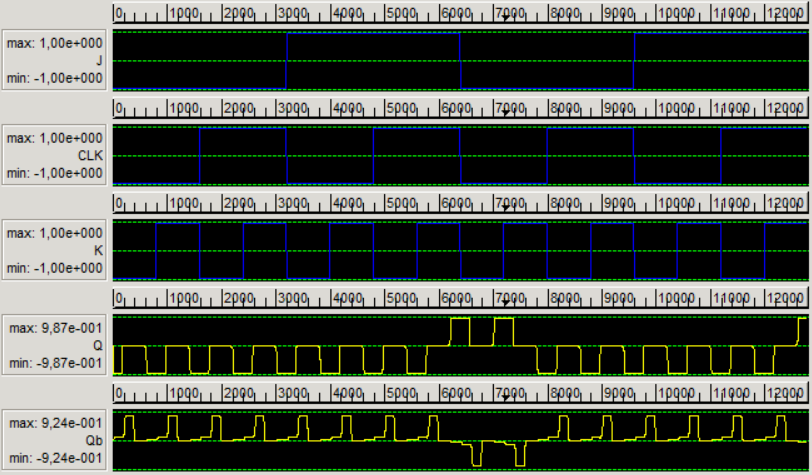
\includegraphics[width=\textwidth]{../img/vir_5/sim_jk.png}
	\caption{Simulacija delovanja JK pomnilne celice po viru \cite{a_novel_approach}}
	\label{fig-jk-2-sim}
	\end{subfigure}
	\caption{Simulaciji JK pomnilne celice}
	\label{fig-jk-sim}
\end{figure}

\subsubsection{RS pomnilna celica}
Pravilnostna tabela RS pomnilne celice je predstavljena v tabeli \ref{tab-rs}.
\begin{table}[h!]
	\centering
	\small
	\begin{tabular}{cc|c}
	$r$ & $s$ & $D^1q$ \\
	\hline
	$0$ & $0$ & $q$ \\
	$0$ & $1$ & $1$ \\
	$1$ & $0$ & $0$ \\
	$1$ & $1$ & $x$ \\
	\end{tabular}
	\caption{Pravilnostna tabela RS pomnilne celice.}
	\label{tab-rs}
\end{table}

Na sliki \ref{fig-rs-sim} vidimo obnašanje $Q$ celice v odvisnosti od vhodov $R$ in $S$ ter urinega signala $Clock$. Iz razbranega lahko sestavimo pravilnostni tabeli \ref{tab-rs-sim}.
\begin{table}[h!]
	\centering
	\small
	\begin{tabular}{ccc|ccccc|c}
	\multicolumn{4}{c}{vir \cite{quantum_dot}} & $\quad$ & \multicolumn{4}{c}{vir \cite{a_novel_approach}}\\
	$S$ & $Clock$ & $R$ & $Q$ && $S$ & $Clock$ & $R$ & $Q$ \\
	\cline{1-4} \cline{6-9}
	$0$ & $0$ & $0$ & $0$ && $0$ & $0$ & $0$ & $1$\\
	$0$ & $0$ & $1$ & $0$ && $0$ & $0$ & $1$ & $0$\\
	$0$ & $1$ & $0$ & $0$ && $0$ & $1$ & $0$ & $0$\\
	$0$ & $1$ & $1$ & $0$ && $0$ & $1$ & $1$ & $0$\\
	$1$ & $0$ & $0$ & $0$ && $1$ & $0$ & $0$ & $0$\\
	$1$ & $0$ & $1$ & $0$ && $1$ & $0$ & $1$ & $0$\\
	$1$ & $1$ & $0$ & $0$ && $1$ & $1$ & $0$ & $0$\\
	$1$ & $1$ & $1$ & $1$ && $1$ & $1$ & $1$ & $1$\\
	\cline{1-4} \cline{6-9}
	$0$ & $0$ & $0$ & $1$ && $0$ & $0$ & $0$ & $1$\\
	$0$ & $0$ & $1$ & $1$ && $0$ & $0$ & $1$ & $0$\\
	$0$ & $1$ & $0$ & $1$ && $0$ & $1$ & $0$ & $0$\\
	$0$ & $1$ & $1$ & $1$ && $0$ & $1$ & $1$ & $0$\\
	$1$ & $0$ & $0$ & $0$ && $1$ & $0$ & $0$ & $0$\\
	$1$ & $0$ & $1$ & $0$ && $1$ & $0$ & $1$ & $0$\\
	$1$ & $1$ & $0$ & $0$ && $1$ & $1$ & $0$ & $0$\\
	$1$ & $1$ & $1$ & $1$ && $1$ & $1$ & $1$ & $1$\\
	\end{tabular}
	\caption{Rezultat simulacije RS pomnilne celice.}
	\label{tab-rs-sim}
\end{table}

\begin{figure}[h!]
	\begin{subfigure}[b]{\textwidth}
	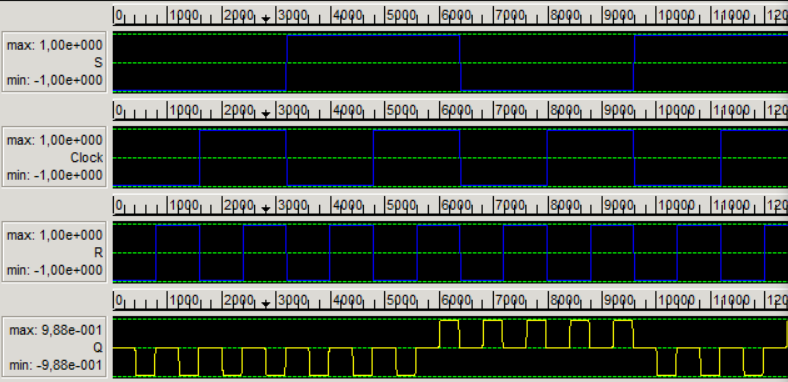
\includegraphics[width=\textwidth]{../img/vir_4/sim_sr.png}
	\caption{Simulacija delovanja RS pomnilne celice po viru \cite{quantum_dot}}
	\label{fig-rs-1-sim}
	\end{subfigure}
	\begin{subfigure}[b]{\textwidth}
	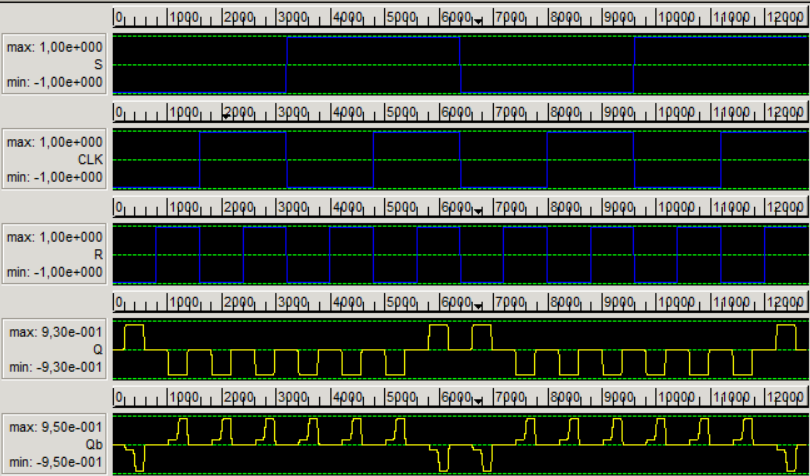
\includegraphics[width=\textwidth]{../img/vir_5/sim_rs.png}
	\caption{Simulacija delovanja RS pomnilne celice po viru \cite{a_novel_approach}}
	\label{fig-rs-2-sim}
	\end{subfigure}
	\caption{Simulaciji RS pomnilne celice}
	\label{fig-rs-sim}
\end{figure}

\subsubsection{T pomnilna celica}
Pravilnostna tabela T pomnilne celice je predstavljena v tabeli \ref{tab-t}.
\begin{table}[h!]
	\centering
	\small
	\begin{tabular}{c|c}
	$t$ & $D^1q$ \\
	\hline
	$0$ & $q$ \\
	$1$ & $\overline{q}$ \\
	\end{tabular}
	\caption{Pravilnostna tabela T pomnilne celice.}
	\label{tab-t}
\end{table}

Na sliki \ref{fig-t-sim} vidimo obnašanje $Q$ celice v odvisnosti od vhoda $T$ in urinega signala $Clock$. Že takoj lahko vidimo, da se rezultata simulacij razlikujeta. Iz razbranega lahko sestavimo pravilnostni tabeli \ref{tab-t-sim}.
\begin{table}[h!]
	\centering
	\small
	\begin{tabular}{cc|cccc|c}
	\multicolumn{3}{c}{vir \cite{quantum_dot}} & $\quad$ & \multicolumn{3}{c}{vir \cite{a_novel_approach}}\\
	$Clock$ & $T$ & $Q$ && $Clock$ & $T$ & $Q$ \\
	\cline{1-3} \cline{5-7}
	$0$ & $0$ & $0$ && $0$ & $0$ & $0$\\
	$0$ & $1$ & $0$ && $0$ & $1$ & $0$\\
	$1$ & $0$ & $0$ && $1$ & $0$ & $0$\\
	$1$ & $1$ & $0$ && $1$ & $1$ & $0$\\
	\cline{1-3} \cline{5-7}
	$0$ & $0$ & $1$ && $0$ & $0$ & $1$\\
	$0$ & $1$ & $1$ && $0$ & $1$ & $0$\\
	$1$ & $0$ & $0$ && $1$ & $0$ & $0$\\
	$1$ & $1$ & $0$ && $1$ & $1$ & $0$\\
	\end{tabular}
	\caption{Rezultat simulacije T pomnilne celice.}
	\label{tab-t-sim}
\end{table}


\begin{figure}[h!]
	\begin{subfigure}[b]{\textwidth}
	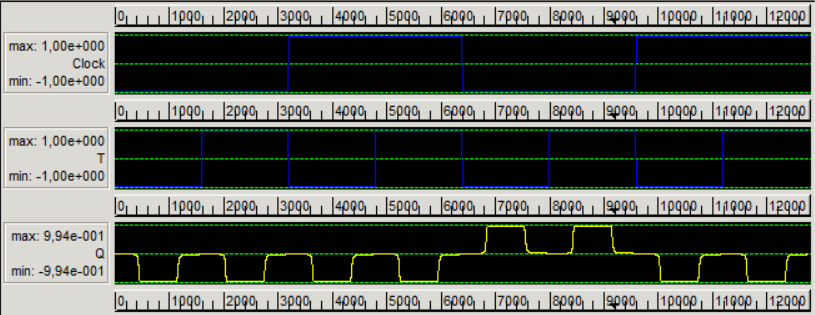
\includegraphics[width=\textwidth]{../img/vir_4/sim_t.png}
	\caption{Simulacija delovanja T pomnilne celice po viru \cite{quantum_dot}}
	\label{fig-t-1-sim}
	\end{subfigure}
	\begin{subfigure}[b]{\textwidth}
	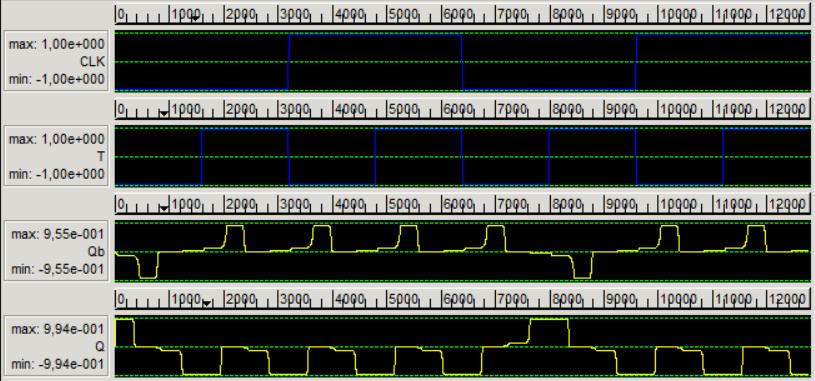
\includegraphics[width=\textwidth]{../img/vir_5/sim_t.png}
	\caption{Simulacija delovanja T pomnilne celice po viru \cite{a_novel_approach}}
	\label{fig-t-2-sim}
	\end{subfigure}
	\caption{Simulaciji T pomnilne celice}
	\label{fig-t-sim}
\end{figure}

\section{Zaključek}
\todo: kratek povzetek glavnih ugotovitev + smernice za nadaljnje delo

\bibliographystyle{babplain}
\bibliography{pomnjenje} 

\end{document}
